\documentclass{standalone}
\usepackage{tikz}
\usetikzlibrary{patterns, positioning}

\begin{document}
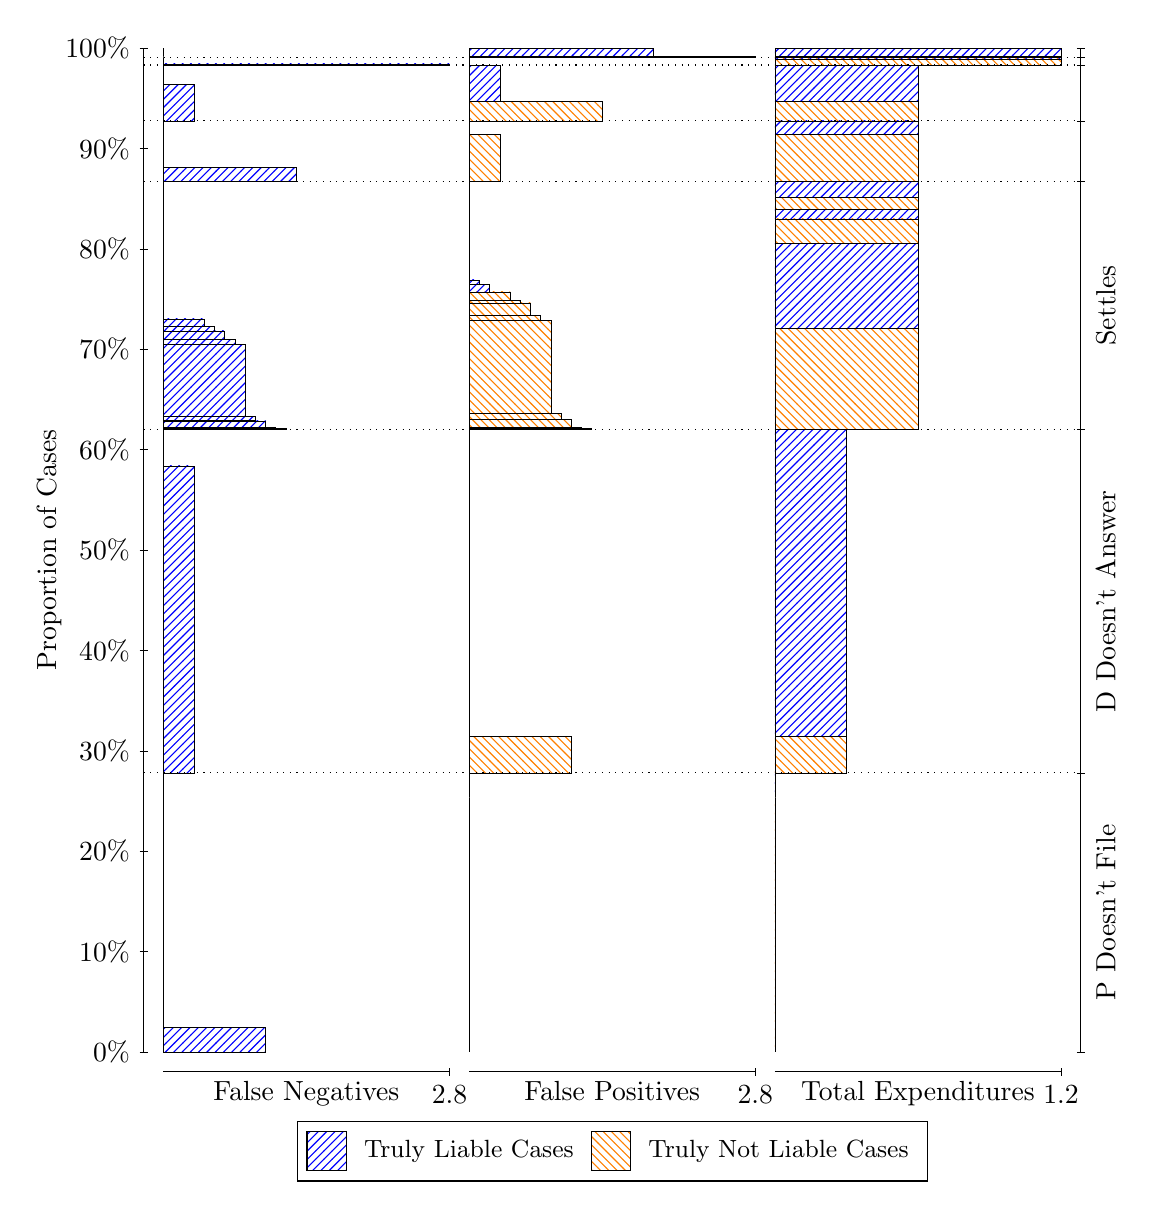
\begin{tikzpicture}
\draw[black, very thin] (1.5,1.75) -- (1.5,14.5);
\node[rotate=90, anchor=center] at (0.3, 8.125) {Proportion of Cases};
\draw[black, very thin] (1.45,1.75) -- (1.55,1.75);
\node[anchor=east] at (1.45, 1.75) {0\%};
\draw[black, very thin] (1.45,3.025) -- (1.55,3.025);
\node[anchor=east] at (1.45, 3.025) {10\%};
\draw[black, very thin] (1.45,4.3) -- (1.55,4.3);
\node[anchor=east] at (1.45, 4.3) {20\%};
\draw[black, very thin] (1.45,5.575) -- (1.55,5.575);
\node[anchor=east] at (1.45, 5.575) {30\%};
\draw[black, very thin] (1.45,6.85) -- (1.55,6.85);
\node[anchor=east] at (1.45, 6.85) {40\%};
\draw[black, very thin] (1.45,8.125) -- (1.55,8.125);
\node[anchor=east] at (1.45, 8.125) {50\%};
\draw[black, very thin] (1.45,9.4) -- (1.55,9.4);
\node[anchor=east] at (1.45, 9.4) {60\%};
\draw[black, very thin] (1.45,10.675) -- (1.55,10.675);
\node[anchor=east] at (1.45, 10.675) {70\%};
\draw[black, very thin] (1.45,11.95) -- (1.55,11.95);
\node[anchor=east] at (1.45, 11.95) {80\%};
\draw[black, very thin] (1.45,13.225) -- (1.55,13.225);
\node[anchor=east] at (1.45, 13.225) {90\%};
\draw[black, very thin] (1.45,14.5) -- (1.55,14.5);
\node[anchor=east] at (1.45, 14.5) {100\%};

\draw[black, very thin] (13.4,1.75) -- (13.4,14.5);
\draw[black, very thin] (13.35,1.75) -- (13.45,1.75);
\node[anchor=west] at (13.35, 1.75) {};
\draw[black, very thin] (13.35,5.2956) -- (13.45,5.2956);
\node[anchor=west] at (13.35, 5.2956) {};
\draw[black, very thin] (13.35,9.6542) -- (13.45,9.6542);
\node[anchor=west] at (13.35, 9.6542) {};
\draw[black, very thin] (13.35,12.809) -- (13.45,12.809);
\node[anchor=west] at (13.35, 12.809) {};
\draw[black, very thin] (13.35,13.574) -- (13.45,13.574);
\node[anchor=west] at (13.35, 13.574) {};
\draw[black, very thin] (13.35,14.284) -- (13.45,14.284);
\node[anchor=west] at (13.35, 14.284) {};
\draw[black, very thin] (13.35,14.377) -- (13.45,14.377);
\node[anchor=west] at (13.35, 14.377) {};
\draw[black, very thin] (13.35,14.5) -- (13.45,14.5);
\node[anchor=west] at (13.35, 14.5) {};

\draw[black, very thin, pattern color=blue, pattern=north east lines] (1.75,1.75) rectangle (3.0476,2.0629);
\draw[black, very thin, pattern color=orange, pattern=north west lines] (1.75,2.0629) rectangle (1.75,5.2956);
\draw[black, very thin, pattern color=blue, pattern=north east lines] (1.75,5.2956) rectangle (2.1393,9.1938);
\draw[black, very thin, pattern color=orange, pattern=north west lines] (1.75,9.1938) rectangle (1.75,9.6542);
\draw[black, very thin, pattern color=blue, pattern=north east lines] (1.75,9.6542) rectangle (3.3071,9.6708);
\draw[black, very thin, pattern color=blue, pattern=north east lines] (1.75,9.6708) rectangle (3.1774,9.6801);
\draw[black, very thin, pattern color=blue, pattern=north east lines] (1.75,9.6801) rectangle (3.0476,9.7636);
\draw[black, very thin, pattern color=blue, pattern=north east lines] (1.75,9.7636) rectangle (2.9179,9.7707);
\draw[black, very thin, pattern color=blue, pattern=north east lines] (1.75,9.7707) rectangle (2.9179,9.8213);
\draw[black, very thin, pattern color=blue, pattern=north east lines] (1.75,9.8213) rectangle (2.7881,10.739);
\draw[black, very thin, pattern color=blue, pattern=north east lines] (1.75,10.739) rectangle (2.6583,10.798);
\draw[black, very thin, pattern color=blue, pattern=north east lines] (1.75,10.798) rectangle (2.5286,10.908);
\draw[black, very thin, pattern color=blue, pattern=north east lines] (1.75,10.908) rectangle (2.3988,10.96);
\draw[black, very thin, pattern color=blue, pattern=north east lines] (1.75,10.96) rectangle (2.269,11.059);
\draw[black, very thin, pattern color=orange, pattern=north west lines] (1.75,11.059) rectangle (1.75,12.809);
\draw[black, very thin, pattern color=blue, pattern=north east lines] (1.75,12.809) rectangle (3.4369,12.984);
\draw[black, very thin, pattern color=orange, pattern=north west lines] (1.75,12.984) rectangle (1.75,13.574);
\draw[black, very thin, pattern color=blue, pattern=north east lines] (1.75,13.574) rectangle (2.1393,14.039);
\draw[black, very thin, pattern color=orange, pattern=north west lines] (1.75,14.039) rectangle (1.75,14.284);
\draw[black, very thin, pattern color=blue, pattern=north east lines] (1.75,14.284) rectangle (5.3833,14.298);
\draw[black, very thin, pattern color=orange, pattern=north west lines] (1.75,14.298) rectangle (1.75,14.377);
\draw[black, very thin, pattern color=orange, pattern=north west lines] (1.75,14.377) rectangle (1.75,14.395);
\draw[black, very thin, pattern color=blue, pattern=north east lines] (1.75,14.395) rectangle (1.75,14.5);
\draw[black, very thin, pattern color=orange, pattern=north west lines] (5.6333,1.75) rectangle (5.6333,4.9827);
\draw[black, very thin, pattern color=blue, pattern=north east lines] (5.6333,4.9827) rectangle (5.6333,5.2956);
\draw[black, very thin, pattern color=orange, pattern=north west lines] (5.6333,5.2956) rectangle (6.931,5.7561);
\draw[black, very thin, pattern color=blue, pattern=north east lines] (5.6333,5.7561) rectangle (5.6333,9.6542);
\draw[black, very thin, pattern color=orange, pattern=north west lines] (5.6333,9.6542) rectangle (7.1905,9.6737);
\draw[black, very thin, pattern color=orange, pattern=north west lines] (5.6333,9.6737) rectangle (7.0607,9.6857);
\draw[black, very thin, pattern color=orange, pattern=north west lines] (5.6333,9.6857) rectangle (6.931,9.7802);
\draw[black, very thin, pattern color=orange, pattern=north west lines] (5.6333,9.7802) rectangle (6.8012,9.8586);
\draw[black, very thin, pattern color=orange, pattern=north west lines] (5.6333,9.8586) rectangle (6.6714,11.04);
\draw[black, very thin, pattern color=orange, pattern=north west lines] (5.6333,11.04) rectangle (6.5417,11.108);
\draw[black, very thin, pattern color=orange, pattern=north west lines] (5.6333,11.108) rectangle (6.4119,11.263);
\draw[black, very thin, pattern color=orange, pattern=north west lines] (5.6333,11.263) rectangle (6.2821,11.299);
\draw[black, very thin, pattern color=orange, pattern=north west lines] (5.6333,11.299) rectangle (6.1524,11.404);
\draw[black, very thin, pattern color=blue, pattern=north east lines] (5.6333,11.404) rectangle (5.8929,11.503);
\draw[black, very thin, pattern color=blue, pattern=north east lines] (5.6333,11.503) rectangle (5.7631,11.555);
\draw[black, very thin, pattern color=blue, pattern=north east lines] (5.6333,11.555) rectangle (5.6333,12.809);
\draw[black, very thin, pattern color=orange, pattern=north west lines] (5.6333,12.809) rectangle (6.0226,13.399);
\draw[black, very thin, pattern color=blue, pattern=north east lines] (5.6333,13.399) rectangle (5.6333,13.574);
\draw[black, very thin, pattern color=orange, pattern=north west lines] (5.6333,13.574) rectangle (7.3202,13.818);
\draw[black, very thin, pattern color=blue, pattern=north east lines] (5.6333,13.818) rectangle (6.0226,14.284);
\draw[black, very thin, pattern color=orange, pattern=north west lines] (5.6333,14.284) rectangle (5.6333,14.363);
\draw[black, very thin, pattern color=blue, pattern=north east lines] (5.6333,14.363) rectangle (5.6333,14.377);
\draw[black, very thin, pattern color=orange, pattern=north west lines] (5.6333,14.377) rectangle (9.2667,14.395);
\draw[black, very thin, pattern color=blue, pattern=north east lines] (5.6333,14.395) rectangle (7.969,14.5);
\draw[black, very thin, pattern color=orange, pattern=north west lines] (9.5167,1.75) rectangle (9.5167,4.9827);
\draw[black, very thin, pattern color=blue, pattern=north east lines] (9.5167,4.9827) rectangle (9.5167,5.2956);
\draw[black, very thin, pattern color=orange, pattern=north west lines] (9.5167,5.2956) rectangle (10.425,5.7561);
\draw[black, very thin, pattern color=blue, pattern=north east lines] (9.5167,5.7561) rectangle (10.425,9.6542);
\draw[black, very thin, pattern color=orange, pattern=north west lines] (9.5167,9.6542) rectangle (11.333,10.942);
\draw[black, very thin, pattern color=blue, pattern=north east lines] (9.5167,10.942) rectangle (11.333,12.021);
\draw[black, very thin, pattern color=orange, pattern=north west lines] (9.5167,12.021) rectangle (11.333,12.331);
\draw[black, very thin, pattern color=blue, pattern=north east lines] (9.5167,12.331) rectangle (11.333,12.447);
\draw[black, very thin, pattern color=orange, pattern=north west lines] (9.5167,12.447) rectangle (11.333,12.6);
\draw[black, very thin, pattern color=blue, pattern=north east lines] (9.5167,12.6) rectangle (11.333,12.809);
\draw[black, very thin, pattern color=orange, pattern=north west lines] (9.5167,12.809) rectangle (11.333,13.399);
\draw[black, very thin, pattern color=blue, pattern=north east lines] (9.5167,13.399) rectangle (11.333,13.574);
\draw[black, very thin, pattern color=orange, pattern=north west lines] (9.5167,13.574) rectangle (11.333,13.818);
\draw[black, very thin, pattern color=blue, pattern=north east lines] (9.5167,13.818) rectangle (11.333,14.284);
\draw[black, very thin, pattern color=orange, pattern=north west lines] (9.5167,14.284) rectangle (13.15,14.363);
\draw[black, very thin, pattern color=blue, pattern=north east lines] (9.5167,14.363) rectangle (13.15,14.377);
\draw[black, very thin, pattern color=orange, pattern=north west lines] (9.5167,14.377) rectangle (13.15,14.395);
\draw[black, very thin, pattern color=blue, pattern=north east lines] (9.5167,14.395) rectangle (13.15,14.5);
\draw[black, dotted] (1.5,5.2956) -- (13.4,5.2956);
\draw[black, dotted] (1.5,9.6542) -- (13.4,9.6542);
\draw[black, dotted] (1.5,12.809) -- (13.4,12.809);
\draw[black, dotted] (1.5,13.574) -- (13.4,13.574);
\draw[black, dotted] (1.5,14.284) -- (13.4,14.284);
\draw[black, dotted] (1.5,14.377) -- (13.4,14.377);
\draw[black, very thin] (1.75,1.5) -- (5.3833,1.5);
\node[anchor=north] at (3.5667, 1.5) {False Negatives};
\draw[black, very thin] (5.3833,1.45) -- (5.3833,1.55);
\node[anchor=north] at (5.3833, 1.45) {2.8};

\draw[black, very thin] (5.6333,1.5) -- (9.2667,1.5);
\node[anchor=north] at (7.45, 1.5) {False Positives};
\draw[black, very thin] (9.2667,1.45) -- (9.2667,1.55);
\node[anchor=north] at (9.2667, 1.45) {2.8};

\draw[black, very thin] (9.5167,1.5) -- (13.15,1.5);
\node[anchor=north] at (11.333, 1.5) {Total Expenditures};
\draw[black, very thin] (13.15,1.45) -- (13.15,1.55);
\node[anchor=north] at (13.15, 1.45) {1.2};

\node[black, centered, rotate=90] at (13.72, 3.5228) {P Doesn't File};
\node[black, centered, rotate=90] at (13.72, 7.4749) {D Doesn't Answer};
\node[black, centered, rotate=90] at (13.72, 11.232) {Settles};





\draw (7.449999999999999,1.5) node[draw=none] (baseCoordinate) {};
\begin{scope}[align=center]
        \matrix[scale=0.5, draw=black, below=0.5cm of baseCoordinate, nodes={draw}, column sep=0.1cm]{
            \node[rectangle, draw, minimum width=0.5cm, minimum height=0.5cm, pattern=north east lines, pattern color=blue] {}; &
            \node[draw=none, font=\small] (B) {Truly Liable Cases}; &
            \node[rectangle, draw, minimum width=0.5cm, minimum height=0.5cm, pattern=north west lines, pattern color=orange] {}; &
            \node[draw=none, font=\small] (B) {Truly Not Liable Cases}; \\
            };
\end{scope}

\end{tikzpicture}
\end{document}